\documentclass[电力电子]{subfiles}
\begin{document}
\section{计算题}
\begin{ti}[10 分]
	调光台灯由单相交流调压电路供电,设该台灯可看作电阻负载,在 $\alpha = 0^\circ$ 时输出功率为最大值,试求功率为最大输出功率的 \SI{80}{\percent} 时的开通角 $\alpha$。
\end{ti}

\begin{ti}[10 分]
	调光台灯由单相交流调压电路供电,设该台灯可看作电阻负载,在 $\alpha = 0^\circ$ 时输出功率为最大值,试求功率为最大输出功率的 \SI{50}{\percent} 时的开通角 $\alpha$。
\end{ti}

\begin{ti}[15 分]
	采用两晶闸管反并联相控的交流调压电路,输入电压 $U_{\ii} = $ \SI{220}{V},负载电阻 $R = $ \SI{5}{\Omega},$L = 0$。如 $\alpha_{1} = \alpha_{2} = \frac{2\uppi}{3}$,求:
	\begin{enumerate}
		\item 试画出输出电压 $u_{\oo}$ 的波形;
		\item 计算输出电压有效值;
		\item 计算晶闸管的平均电流。
	\end{enumerate}
\end{ti}

\begin{ti}[16 分]
	一个电炉由单相交流调压电路供电,$\alpha = 0^\circ$ 时输出功率为最大值。
	\begin{enumerate}
		\item 试求输出功率为最大值的 \SI{50}{\percent} 的控制角 $\alpha$ 和输出功率为零时的控制角 $\alpha$;
		\item 画出输出 $u_{\oo},i_{\oo},u_{\mathrm{vt}}$ 的电压波形。
	\end{enumerate}
\end{ti}

\begin{ti}
	一个电炉由单相交流调压电路供电,$\alpha = 0^\circ$ 时输出功率为最大值,试求输出功率为最大值的 \SI{80}{\percent} 的控制角 $\alpha$ 和输出功率为零时的控制角 $\alpha$。
\end{ti}

\begin{ti}
	单相全控桥式整流电路接大电感负载。已知:$U_{2} = $ \SI{220}{V},$R = $ \SI{10}{\Omega},$\alpha = 60^\circ$。
	\begin{enumerate}
		\item 计算整流输出电压 $U_{\dd}$、整流输出电流的平均值 $I_{\dd}$;
		\item 计算流过晶闸管电流的有效值 $I_{\V}$。
	\end{enumerate}
\end{ti}

\begin{ti}[18 分]
	单相全控桥式整流电路接大电感负载。已知:$U_{2} = $ \SI{220}{V},$R = $ \SI{10}{\Omega},$\alpha = 60^\circ$。
	\begin{enumerate}
		\item 计算整流输出电压 $U_{\dd}$、整流输出电流的平均值 $I_{\dd}$;
		\item 计算流过晶闸管电流的有效值 $I_{\V}$;
		\item 画出输出电压 $u_{\dd}$ 的波形和流过晶闸管 \V 的电流 $i_{\V}$ 波形。
	\end{enumerate}
\end{ti}

\begin{ti}[10 分]
	三相全控桥式有源逆变电路如图所示,变压器二次相电压的有效值 $U_{2} = $ \SI{220}{V},回路总电阻 $R_{\sum} = $ \SI{0.5}{\Omega},平波电抗器 $L$ 足够大,可使负载电流连续,若 $E_{\dd} = $ \SI{-280}{V},要求电机在制动过程中的负载电流 $I_{\dd} = $ \SI{45.2}{A},试回答下列各题:
	\begin{enumerate}
		\item 求出此时的逆变控制角 $\beta$;
		\item 计算变压器二次电流的有效值 $I_{2}$,计算变压器二次的总容量 $S_{2}$。
	\end{enumerate}
\end{ti}

\begin{ti}[10 分]
	有一个三相全控桥整流电路如图所示。已知电感负载 $L = \SI{0.2}{H}$、$\alpha = 75^\circ$、$R = \SI{1}{\Omega}$、变压器二次相电压 $U_{2} = \SI{100}{V}$。试画出 $u_{\dd}$ 的波形,计算负载的平均整流电压 $U_{\dd}$ 和负载电流平均值 $I_{\dd}$,计算变压器二次电流的有效值 $I_{2}$。
\end{ti}

\begin{ti}[10 分]
	一台工业炉原由额定电压为单相交流 \SI{220}{V} 供电,额定功率为 $10$ 千瓦。现改用双向晶闸管组成的单相交流调压电源供电,如果正常工作时负载只需要 $5$ 千瓦。试问双向晶闸管的触发角 $\alpha$ 应为多少度?试求此时的电流有效值,以及电源侧的功率因数值。
\end{ti}

\begin{ti}[10 分]
	一台工业炉原由额定电压为单相交流 \SI{220}{V} 供电,额定功率为 $10$ 千瓦。现改用双向晶闸管组成的单相交流调压电源供电,如果正常工作时负载只需要 $5$ 千瓦。试问双向晶闸管的触发角 $\alpha$ 应为多少度?试求此时的电流有效值,以及电源侧的功率因数值。
\end{ti}

\begin{ti}[10 分]
	三相半波可控整流电路,变压器二次相电压为 \SI{20}{V},带大电感负载,无续流二极管,试计算 $\alpha = 45^\circ$ 时输出电压,如负载为 \SI{200}{A},求晶闸管上最高电压和晶闸管电流的平均值 $I_{\dd \mathrm{T}}$、有效值 $I_{\mathrm{T}}$。
\end{ti}

\begin{ti}[15 分]
	单相全控桥式变流电路如图所示,工作于有源逆变状态,$\beta = 60^\circ$,变压器二次相电压有效值 $U_{2} = \SI{220}{V}$,$E_{\dd} = - \SI{150}{V}$,$R = \SI{1}{\Omega}$,$L$ 足够大,试按要求完成下列各项:
	\begin{enumerate}
		\item 画出输出电压 $u_{\dd}$ 的波形;
		\item 画出输出电流 $i_{\dd}$ 的波形;
		\item 计算输出电流平均值 $I_{\dd}$;
		\item 计算晶闸管电流的平均值 $I_{\dd \mathrm{V}_{1}}$ 和有效值 $I_{\mathrm{V}_{1}}$。
	\end{enumerate}
\end{ti}

\begin{ti}[15 分]
	单相半波可控整流电路对电感负载,$L = \SI{20}{mH}$,$U_{2} = \SI{100}{V}$,求当 $\alpha = 0^\circ$ 时的负载电流 $I_{\dd}$,并画出 $u_{\dd}$ 和 $i_{\dd}$ 的波形。
\end{ti}

\begin{ti}[10 分]
	采用两晶闸管反并联相控的单相调压电路,输入为市电,负载为 RL 串联,$R = \SI{1}{\ohm}$,$L = \SI{5.5}{mH}$。求:
	\begin{enumerate}
		\item 控制角移相范围;
		\item 负载电流最大值;
		\item 最大输出功率;
		\item 最大功率因数。
	\end{enumerate}
\end{ti}

\begin{ti}[10 分]
	采用两晶闸管反并联相控的单相调压电路,输入为市电,负载为 RL 串联,$R = \SI{1}{\ohm}$,$L = \SI{5.5}{mH}$。求:
	\begin{enumerate}
		\item 控制角移相范围;
		\item 负载电流最大值;
		\item 最大输出功率;
		\item 最大功率因数。
	\end{enumerate}
\end{ti}

\begin{ti}[10 分]
	如图所示斩波电路,直流电源电压 $E = \SI{100}{V}$,斩波频率 $f = \SI{1}{kHz}$。若要求输出电压 $u_{\dd}$ 的平均值 $= \SI{25}{V} \sim \SI{75}{V}$ 可调,试计算斩波器 V 的占空比 $\alpha$ 的变化范围以及相应的斩波器 V 的导通时间 $t_{\mathrm{on}}$ 的变化范围。
	\begin{center}
		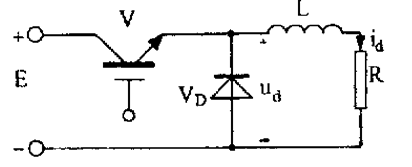
\includegraphics[width=0.5\textwidth]{figure/fig13.png}
	\end{center}
\end{ti}

\begin{ti}[10 分]
	一单相交流调压器,电源为工频 \SI{220}{V},阻感串联作为负载,其中 $R = \SI{1}{\ohm}$,$L = \SI{2}{mH}$。试求:
	\begin{enumerate}
		\item 开通角 $\alpha$ 的变化范围;
		\item 负载电流的最大有效值;
		\item 最大输出功率及此时电源侧的功率因数。
	\end{enumerate}
\end{ti}

\begin{ti}[10 分]
	单相全控桥式整流电路接大电感负载。已知 $R = \SI{10}{\ohm}$,$\alpha = 45^\circ$,$U_{2} = \SI{100}{V}$,试回答:
	\begin{enumerate}
		\item 计算输出整流电压 $U_{\dd}$、输出电流平均值 $I_{\dd}$;
		\item 计算晶闸管电流的有效值 $I_{\mathrm{V}_{1}}$;
		\item 按裕量系数 2 确定晶闸管的额定电流。
	\end{enumerate}
\end{ti}
\end{document}